\documentclass[a4paper]{scrartcl}
\pdfinfoomitdate=1
\pdftrailerid{}
\author{Angewandte Informatik}
\title{Grundlagen der Informatik}
%Language specific formating options
\usepackage[utf8]{inputenc} % use utf8 file encoding for TeX sources
\usepackage[T1]{fontenc}    % avoid garbled Unicode text in pdf
\usepackage[english]{babel} % english grammar so words can go in two lines  
\usepackage{graphicx}
\graphicspath{ {./images/} }
\usepackage{multirow}
\usepackage{longtable}
\usepackage{amsmath}
\usepackage{circuitikz}
\date{WS 20/21}
\begin{document}
    \section{misc}
    \subsection{ASCII table}
        \centering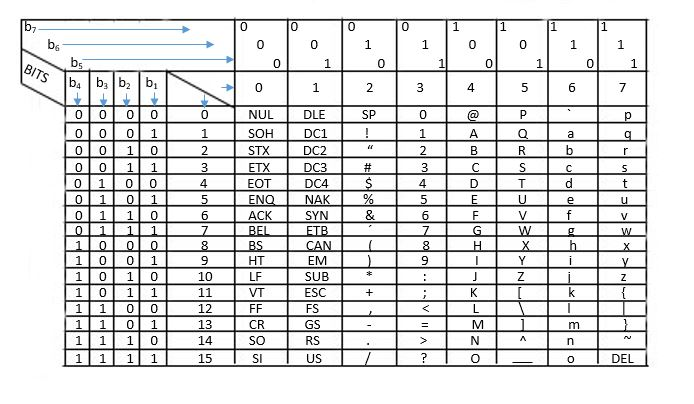
\includegraphics[scale=1.1]{ascii1.png}
    \subsection{ARM ISA}
        \subsubsection{ARM Assembler Commands}
        \centering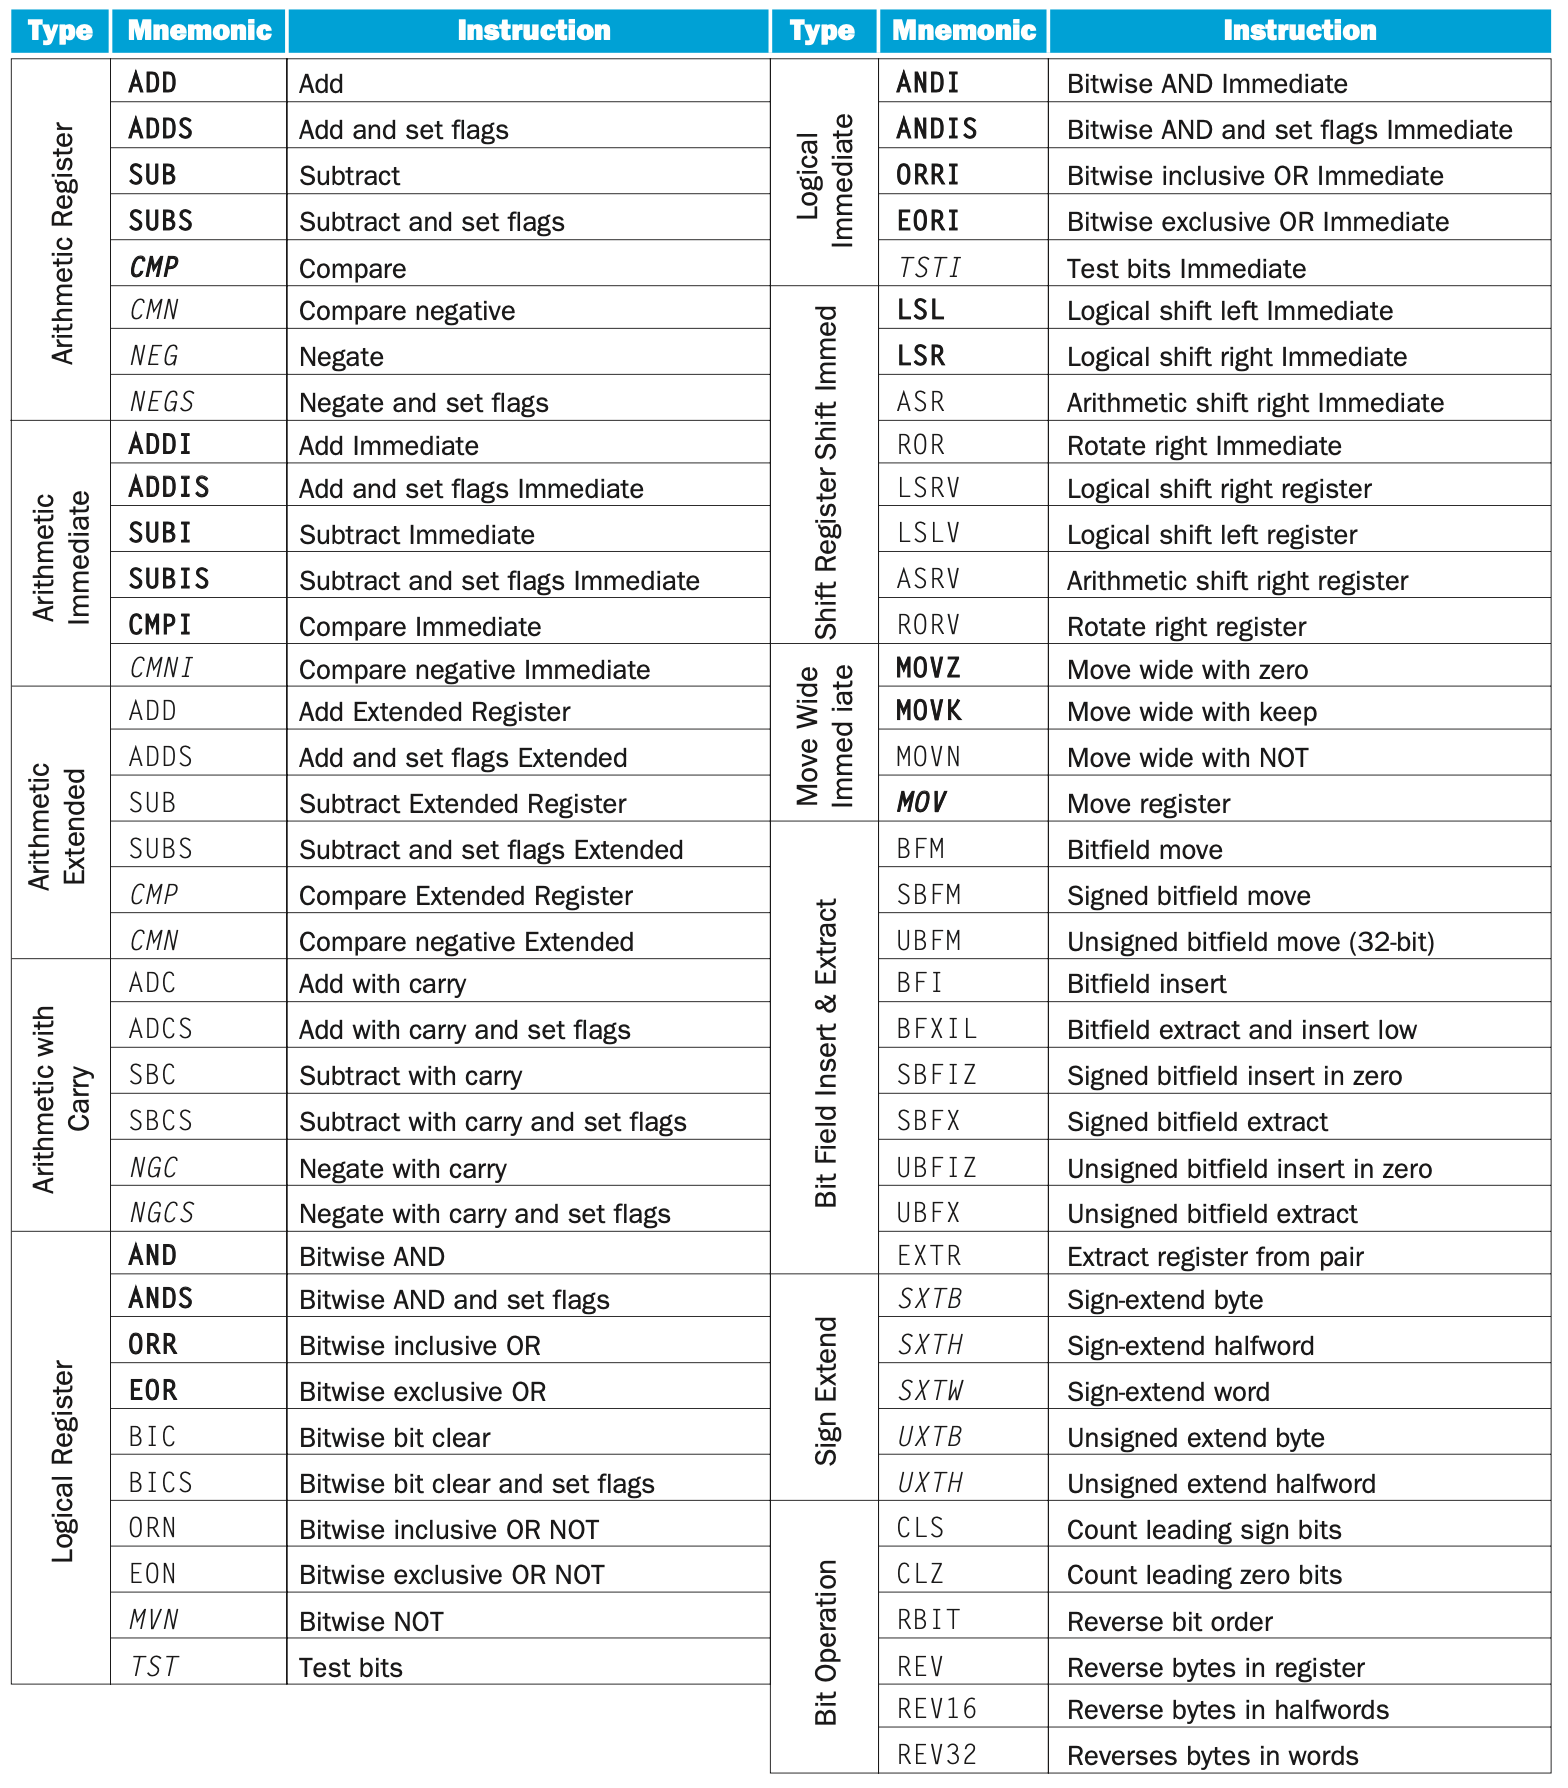
\includegraphics[scale=0.25]{arm_assembler1.png}
        \centering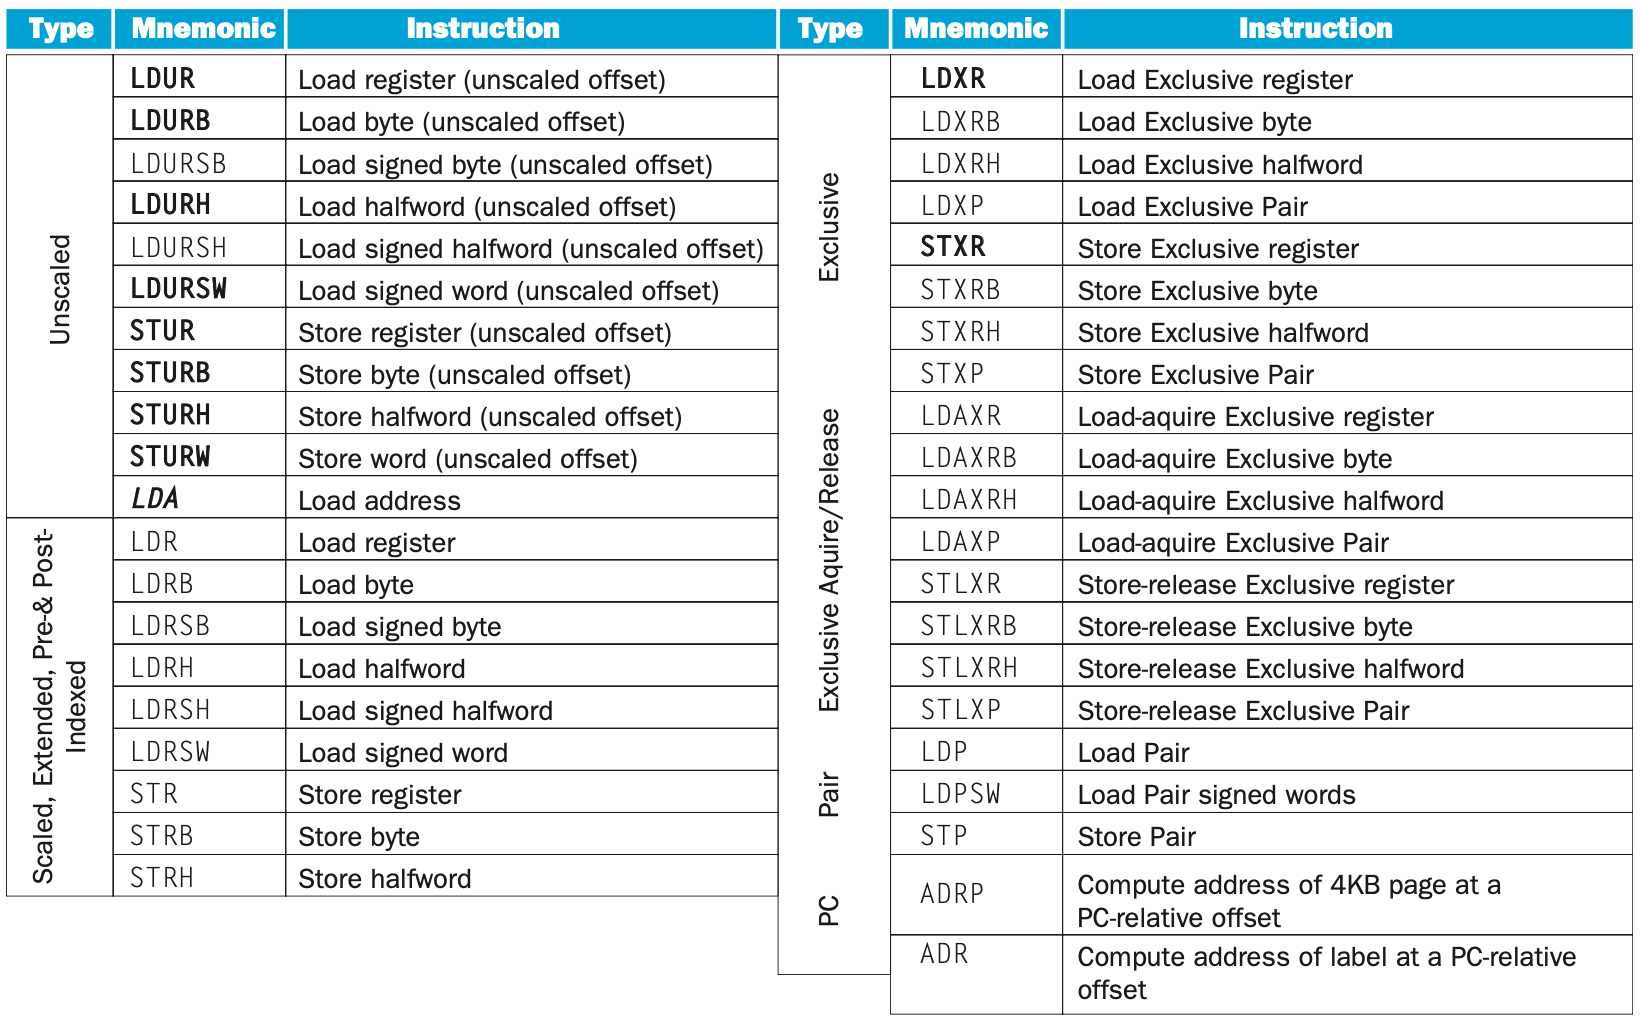
\includegraphics[scale=0.25]{arm_assembler2.png}
        \centering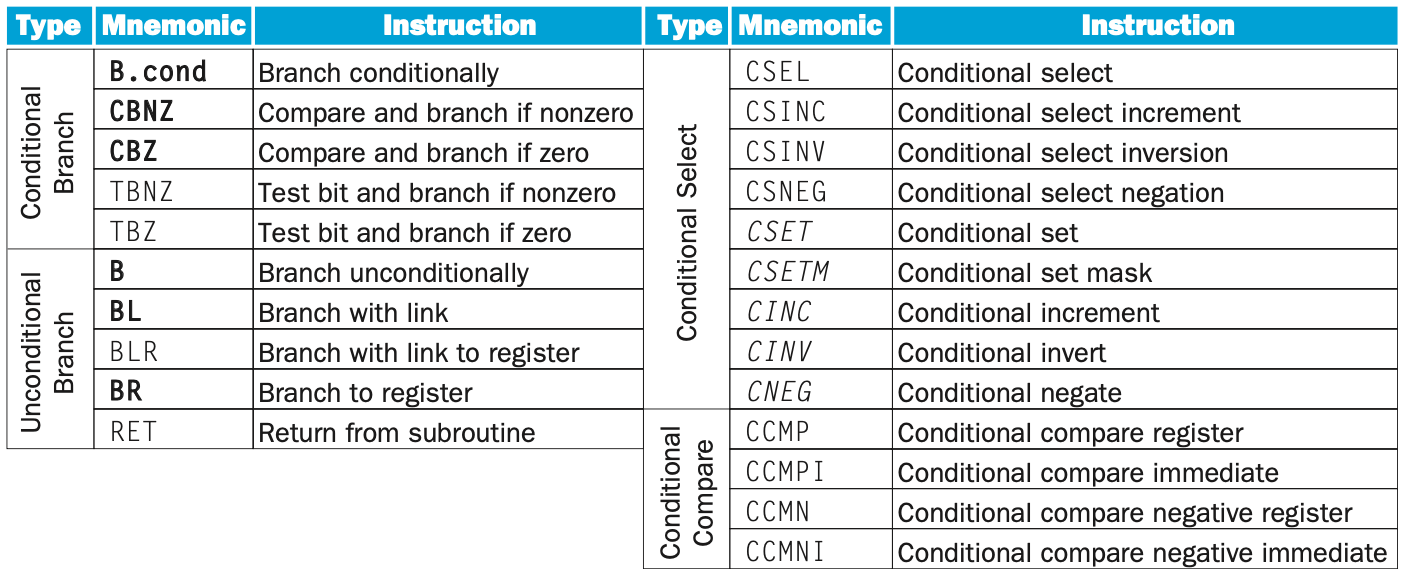
\includegraphics[scale=0.3]{arm_assembler3.png} 
        \centering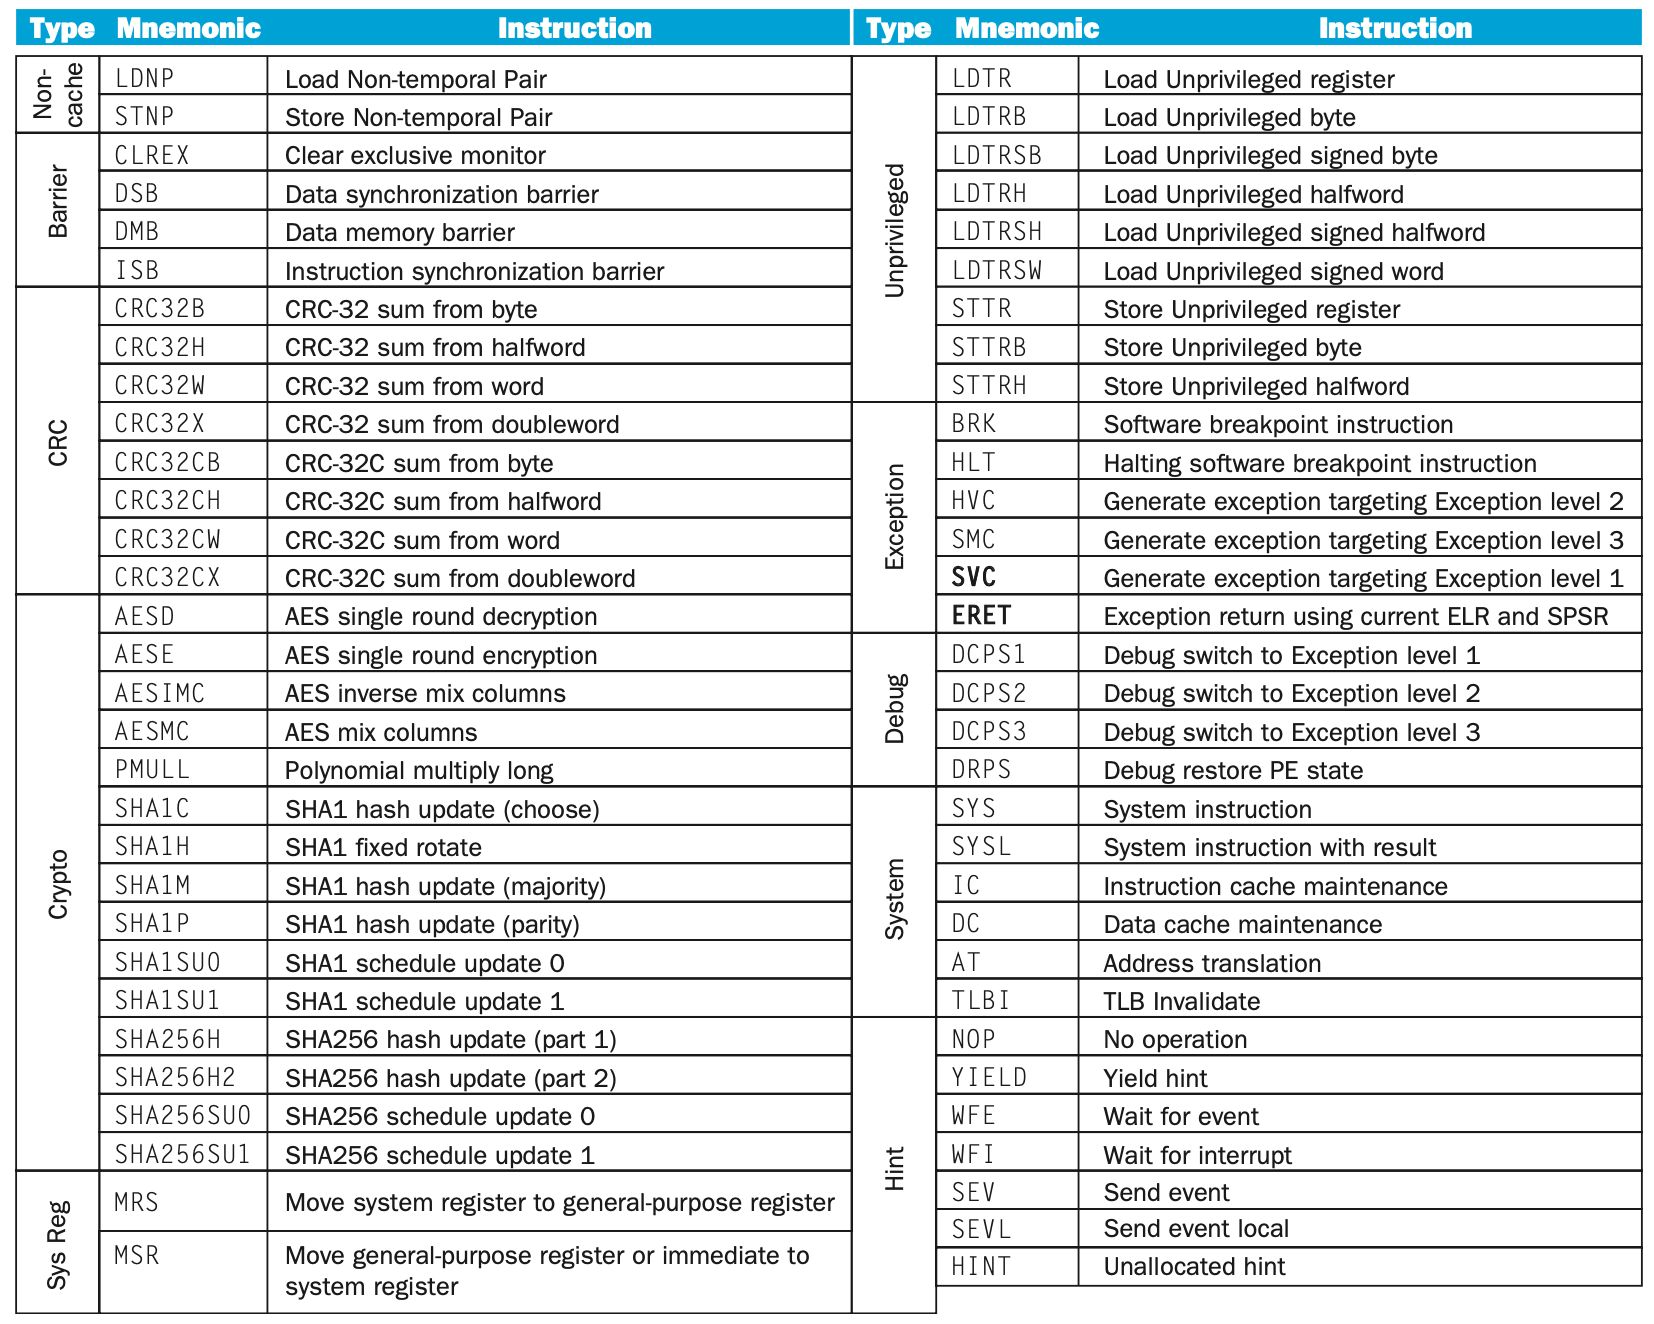
\includegraphics[scale=0.26]{arm_assembler4.png}
        \subsubsection{Opcode}
        \centering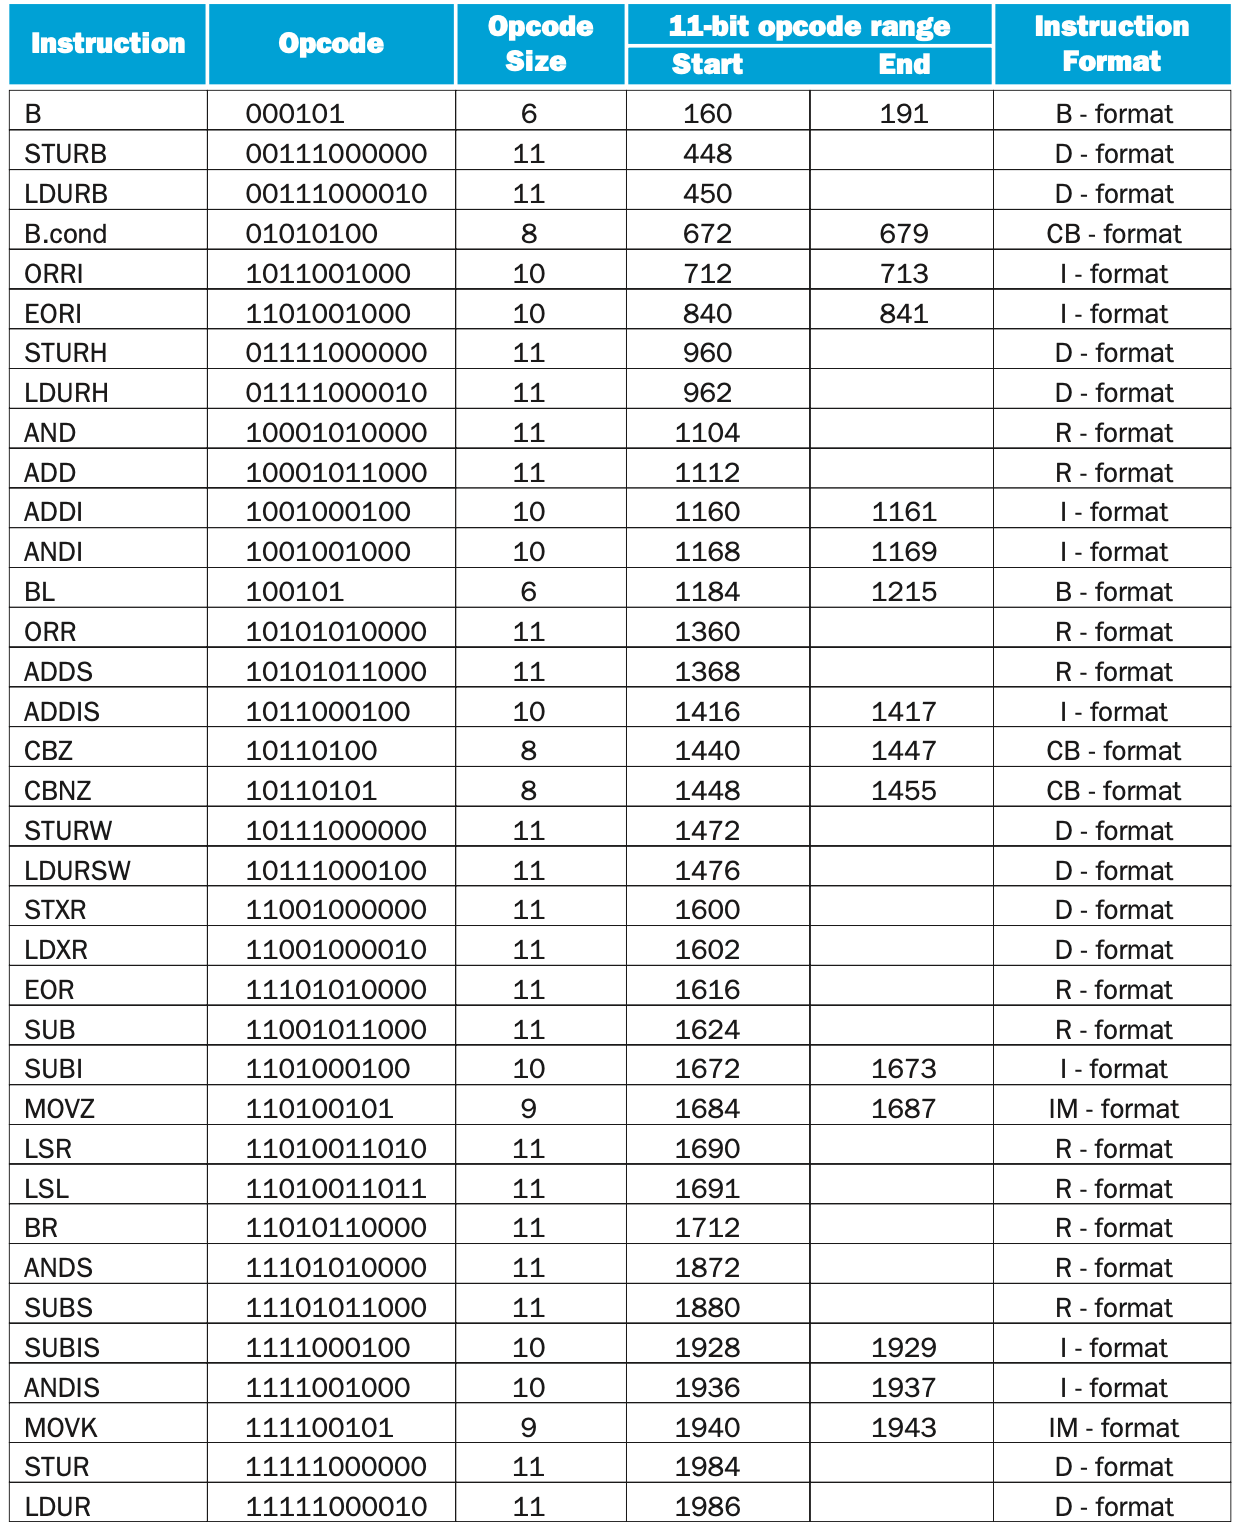
\includegraphics[scale=0.26]{opcode.png}
    \subsection{ARM buses}
        \subsubsection{AHB/AMBA signals}
        \subsubsection*{AHB bus signals}
        \centering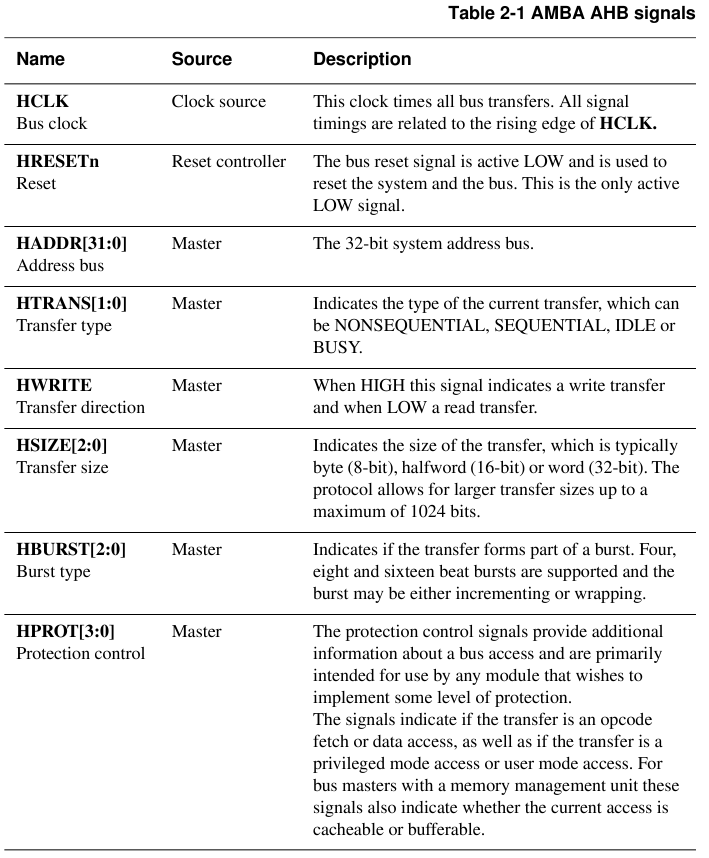
\includegraphics[scale=0.4]{amba1.png}
        \subsubsection*{Read/Write bus signals}
        \centering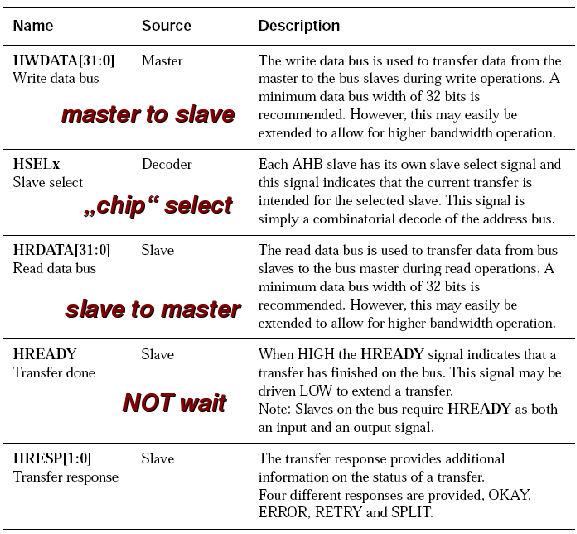
\includegraphics[scale=0.6]{amba2.png}
        \subsubsection*{Arbitration signals}
        \centering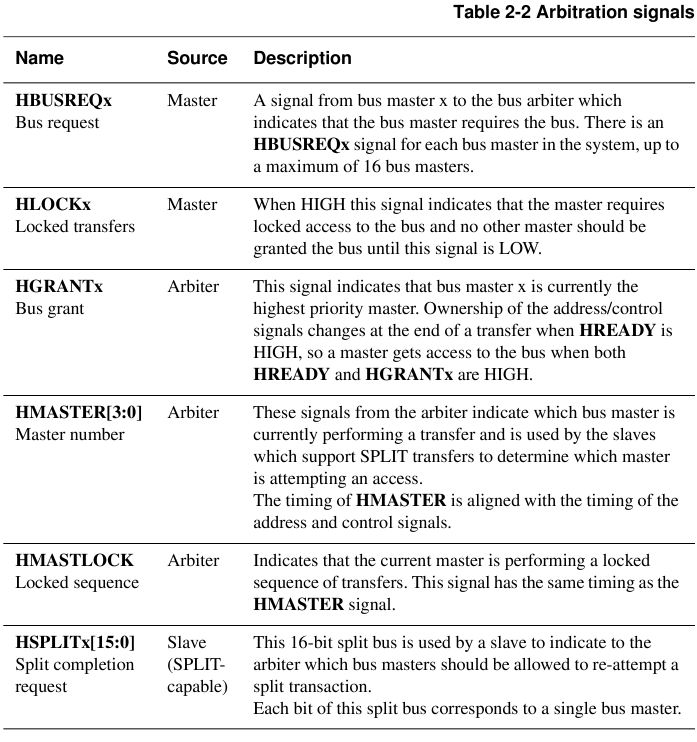
\includegraphics[scale=0.6]{amba3.png}
        \subsubsection*{APB signals}
        \centering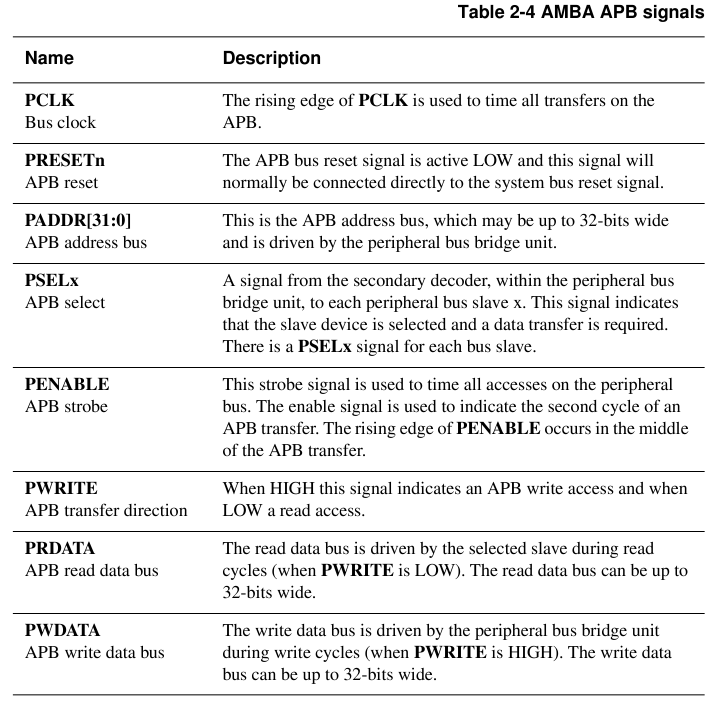
\includegraphics[scale=0.6]{amba4.png}
        \subsubsection*{AHB burst signals}
        \centering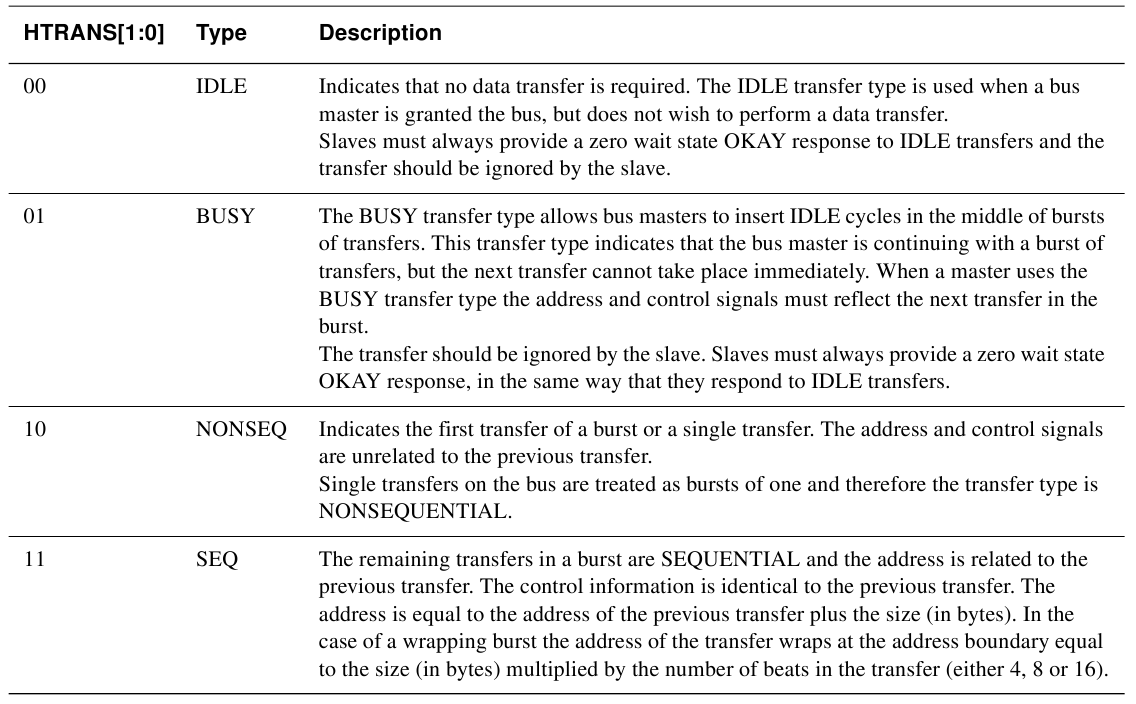
\includegraphics[scale=0.4]{amba6.png}
        \subsubsection*{size and beats of burst}
        \centering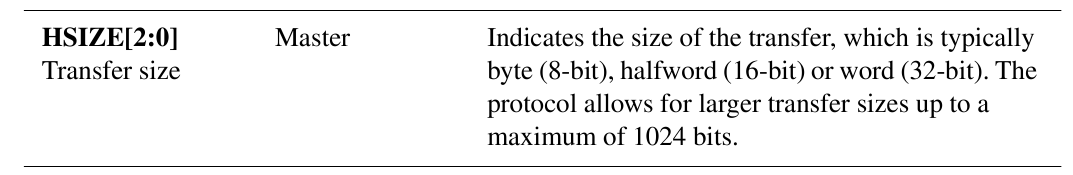
\includegraphics[scale=0.4]{amba8.png}
        \centering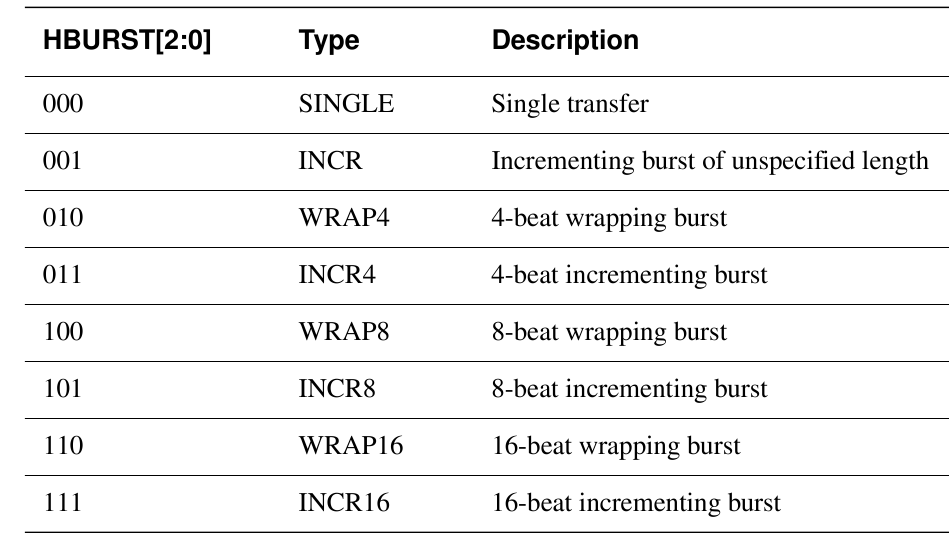
\includegraphics[scale=0.4]{amba9.png}
        \subsubsection*{Slave response signals}
        \centering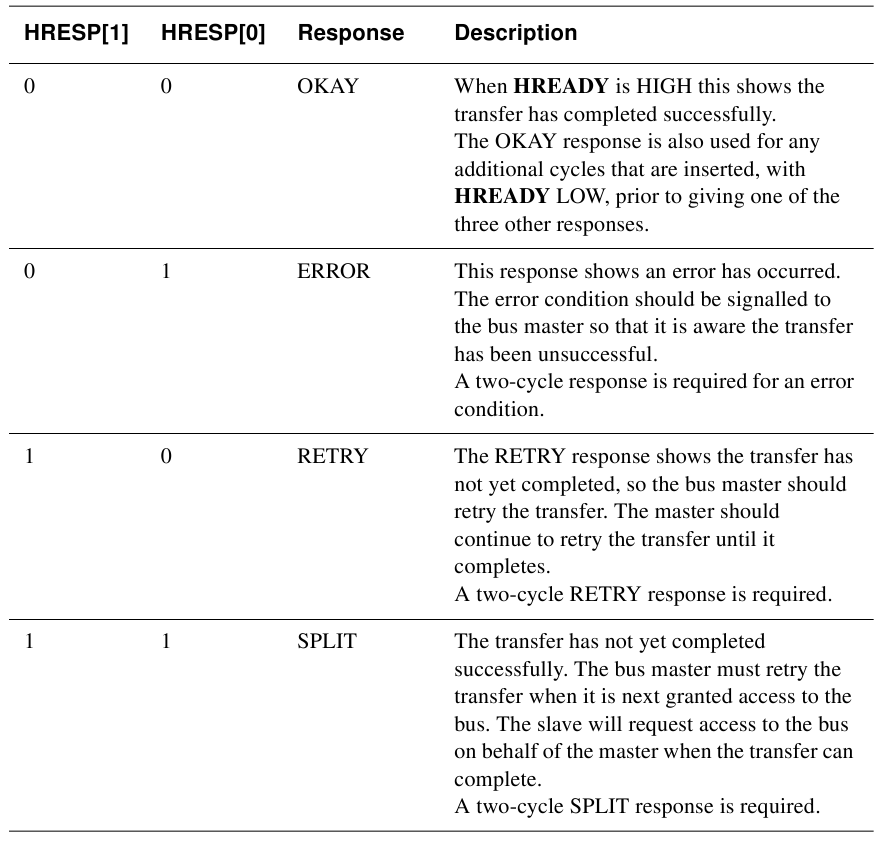
\includegraphics[scale=0.4]{amba10.png}
        \subsubsection{AXI}
        \subsubsection*{Read/write adress-channel signals\footnote{Descriptions shorted so table can fit on screen}}
        \begin{longtable}[c]{| l | c | c |} 
            \hline
            Signal description & Write addr. ch. & Read addr. ch. \\ \hline \hline
            Address ID & AWID & ARID \\ \hline
            Address of the first beat of the burst & AWADDR & ARADDR \\ \hline
            Number of beats inside the burst & AWLEN & ARLEN \\\hline
            Size of each beat &   AWSIZE & ARSIZE \\ \hline
            Type of the burst &
            AWBURST &
            ARBURST \\ \hline
            Lock type, to provide atomic operations  &
            AWLOCK &
            ARLOCK \\ \hline
            Memory type&
            AWCACHE &
            ARCACHE \\ \hline
            Protection type &
            AWPROT &
            ARPROT \\ \hline
            Quality of Service of the transaction &
            AWQOS &
            ARQOS \\ \hline
            Region identifier &
            AWREGION &
            ARREGION \\ \hline
            User-defined data &
            AWUSER &
            ARUSER \\ \hline
            xVALID handshake signal &
            AWVALID &
            ARVALID \\ \hline
            xREADY handshake signal &
            AWREADY &
            ARREADY \\ \hline
        \end{longtable}\subsubsection*{Read/Write data-channel signals}
        \begin{longtable}[c]{| l | c | c |} 
            \hline
            Signal description &
            Write dat. ch. &
            Read dat. ch. \\ \hline \hline
            Data ID, to identify multiple streams over a
            single channel &
            WID &
            RID \\ \hline
            Read/Write data &
            WDATA &
            RDATA \\ \hline
            Read response, status of the current RDATA signal &
            - &
            RRESP \\ \hline
            Byte strobe, which bytes of WDATA are valid  &
            WSTRB &
            - \\ \hline
            Last beat identifier &
            WLAST &
            RLAST \\ \hline
            User-defined data &
            WUSER &
            RUSER \\ \hline
            xVALID handshake signal &
            WVALID &
            RVALID \\ \hline
            xREADY handshake signal &
            WREADY &
            RREADY \\ \hline
        \end{longtable}
        \subsubsection*{Write response signals}
        \begin{longtable}[c]{| l | c |}
            \hline
            Signal description &
            Write resp. ch. \\ \hline
            Write response ID &
            BID \\ \hline
            Write response, to specify the status of the burst &
            BRESP \\ \hline
            User-defined data &
            BUSER \\ \hline
            xVALID handshake signal &
            BVALID \\ \hline
            xREADY handshake signal &
            BREADY \\ \hline
        \end{longtable} 
        \subsubsection*{Slave response channel (uses write repsonse channel)}
        \begin{longtable}[l]{|l|l|}
            \hline
            OKAY &  
            \. The answer of the slave if a normal access has been successful.\\ \hline 
            EXOKAY  &
            \begin{tabular}{l}
                The answer of the slave if a normal exclusive access has been \\
            successful. An exclusive access is an access where only one master \\
            is allowed to access this slave. It is not required, that the bus is \\
            occupied the whole time. 
            \end{tabular} \\ \hline
            SLVERR & 
            This error will be set, when the transaction has been faulty. \\ \hline
            DECERR   &
            \begin{tabular}{l}
                This error will be signalled by the interconnect to the  master if it \\ couldn't find the slave under the given adress.
            occupied the whole time. 
            \end{tabular} \\ \hline
        \end{longtable}
        \newpage
        \subsubsection{Burst}
        \begin{longtable}[c]{|l|c|}
            \hline
            ARBURST[1:0], AWBURST[1:0] &
            Burst Type \\ \hline 
            \(00_2\) &
            FIXED \\ \hline
            \(01_2\) &
            INCR \\ \hline
            \(10_2\) &
            WRAP \\ \hline
            \(11_2\) &
            Reserved \\ \hline \hline
            ARSIZE[2:0], AWSIZE[2:0] & Bytes in transfer \\ \hline 
            3 bits & 1 - 128 (\(2^{ARSIZE/AWSIZE}\)) \\ \hline \hline
            ARLEN[3:0], AWLEN[3:0] & Number of data transfers \\ \hline
            4 bits & 1 - 16 (\(2^{1 - 4}\)) \\
            \hline
        \end{longtable}



        

\end{document}